% --------------------------------------------------------------------------- %
% Poster for the ECCS 2011 Conference about Elementary Dynamic Networks.      %
% --------------------------------------------------------------------------- %
% Created with Brian Amberg's LaTeX Poster Template. Please refer for the     %
% attached README.md file for the details how to compile with `pdflatex`.     %
% --------------------------------------------------------------------------- %
% $LastChangedDate:: 2011-09-11 10:57:12 +0200 (V, 11 szept. 2011)          $ %
% $LastChangedRevision:: 128                                                $ %
% $LastChangedBy:: rlegendi                                                 $ %
% $Id:: poster.tex 128 2011-09-11 08:57:12Z rlegendi                        $ %
% --------------------------------------------------------------------------- %
\documentclass[a0paper,portrait]{baposter}
\usepackage{relsize}		% For \smaller
\usepackage{url}			% For \url
\usepackage{epstopdf}	% Included EPS files automatically converted to PDF to include with pdflatex
\usepackage{lipsum}	% generate non sense text to fill boxes
\usepackage[export]{adjustbox}
\usepackage{enumitem}
\usepackage[none]{hyphenat}

%%% Global Settings %%%%%%%%%%%%%%%%%%%%%%%%%%%%%%%%%%%%%%%%%%%%%%%%%%%%%%%%%%%

\graphicspath{{pix/}}	% Root directory of the pictures
\tracingstats=2			% Enabled LaTeX logging with conditionals

%%% Color Definitions %%%%%%%%%%%%%%%%%%%%%%%%%%%%%%%%%%%%%%%%%%%%%%%%%%%%%%%%%

\definecolor{bordercol}{RGB}{40,40,40}
\definecolor{headercol1}{RGB}{28,144,153}
\definecolor{headercol2}{RGB}{80,80,80}
\definecolor{headerfontcol}{RGB}{0,0,0}
\definecolor{boxcolor}{RGB}{255,255,255} % white

%%%%%%%%%%%%%%%%%%%%%%%%%%%%%%%%%%%%%%%%%%%%%%%%%%%%%%%%%%%%%%%%%%%%%%%%%%%%%%%%
%%% Utility functions %%%%%%%%%%%%%%%%%%%%%%%%%%%%%%%%%%%%%%%%%%%%%%%%%%%%%%%%%%

%%% Save space in lists. Use this after the opening of the list %%%%%%%%%%%%%%%%
\newcommand{\compresslist}{
	\setlength{\itemsep}{1pt}
	\setlength{\parskip}{0pt}
	\setlength{\parsep}{0pt}
}

%%%%%%%%%%%%%%%%%%%%%%%%%%%%%%%%%%%%%%%%%%%%%%%%%%%%%%%%%%%%%%%%%%%%%%%%%%%%%%%
%%% Document Start %%%%%%%%%%%%%%%%%%%%%%%%%%%%%%%%%%%%%%%%%%%%%%%%%%%%%%%%%%%%
%%%%%%%%%%%%%%%%%%%%%%%%%%%%%%%%%%%%%%%%%%%%%%%%%%%%%%%%%%%%%%%%%%%%%%%%%%%%%%%

\begin{document}
\typeout{Poster rendering started}

%%% General Poster Settings %%%%%%%%%%%%%%%%%%%%%%%%%%%%%%%%%%%%%%%%%%%%%%%%%%%
%%%%%% Eye Catcher, Title, Authors and University Images %%%%%%%%%%%%%%%%%%%%%%
\begin{poster}{
	grid=false,
	columns=5,
	% Option is left on true though the eyecatcher is not used. The reason is
	% that we have a bit nicer looking title and author formatting in the headercol
	% this way
	%eyecatcher=false,
	borderColor=bordercol,
	headerColorOne=headercol1!70,%blue!20,
	headerColorTwo=headercol1!70,%blue!20,
	headerFontColor=headerfontcol,
	% Only simple background color used, no shading, so boxColorTwo isn't necessary
	boxColorOne=boxcolor,
	headershape=roundedright,
	headerfont=\large\sf\bf,
	textborder=faded,%rectangle,
	headerborder=open,
  	boxshade=plain,
	background=plain,
	bgColorOne=white,
	bgColorTwo=red,
	headerheight=6cm
}
%%% Eye Cacther %%%%%%%%%%%%%%%%%%%%%%%%%%%%%%%%%%%%%%%%%%%%%%%%%%%%%%%%%%%%%%%
{

	
\includegraphics[width=3cm]{figures/Max-Planck-Gesellschaft.png}

}
%%% Title %%%%%%%%%%%%%%%%%%%%%%%%%%%%%%%%%%%%%%%%%%%%%%%%%%%%%%%%%%%%%%%%%%%%%
{\Large\bf
	mitoBench \& mitoDB: Novel interactive methods for population genetics on mitochondrial DNA
}
%%% Authors %%%%%%%%%%%%%%%%%%%%%%%%%%%%%%%%%%%%%%%%%%%%%%%%%%%%%%%%%%%%%%%%%%%
{
	\vspace{1em} Alexander Peltzer$^{1,2*}$, Judith Neukamm$^{1,3*}$, The mitoDB project consortium$^\dagger$,\\ Kay Nieselt$^{1}$ and Wolfgang Haak$^{2}$\\
	{\footnotesize \textit{$^1$ Integrative Transcriptomics, Center for Bioinformatics (ZBIT), University of Tuebingen, Germany.\\
	$^2$ Max Planck Institute for the Science of Human History, Jena, Germany.\\
	$^3$ Institute for Archaeological Sciences, Archaeo- and Paleogenetics, University of Tuebingen, Germany.\\
	$\dagger$ See \url{http://bit.ly/2vB8wKx} for full author-list.}\\
	$*$These authors contributed equally to the work. \\
	\vspace{1em}
	Contact: peltzer@shh.mpg.de, judith.neukamm@uni-tuebingen.de
	}
}
%%% Logo %%%%%%%%%%%%%%%%%%%%%%%%%%%%%%%%%%%%%%%%%%%%%%%%%%%%%%%%%%%%%%%%%%%%%%
{
% The logos are compressed a bit into a simple box to make them smaller on the result

\begin{minipage}{0.15\textwidth}
	\begin{center}
		
\includegraphics[width=3cm]{figures/Tuebingen.png}
		%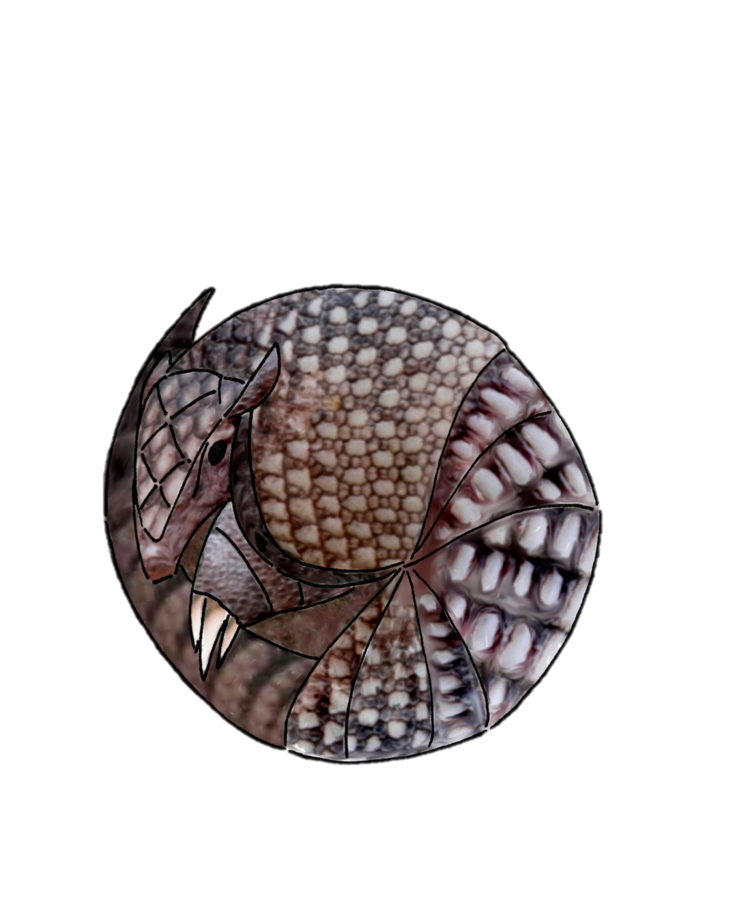
\includegraphics[width=2.5cm]{figures/Pali.png}
	\end{center}
\end{minipage}

}



%---------------------------------------Ha-------------------------------------------------
%	Introduction
%----------------------------------------------------------------------------------------

\headerbox{Motivation \& Goals}{name=introduction, row=0, column=0, span=5}{
		\begin{itemize}[leftmargin=*]
				\item Mitochondrial DNA (mtDNA) is often the only proxy available to study extinct populations and their relationship with modern populations
				\item Tools for the analysis typically rely on different file formats $\rightarrow$ requiring manual interaction with the data for downstream analysis
				\item mitoBench: workbench to ease file conversions, methods to interactively analyze and visualize human mitochondrial data
				\item mitoDB: database for human mitochondrial genomes to provide a central reference that can be easily accessed via the workbench and a web-frontend
		\end{itemize}

}


%----------------------------------------------------------------------------------------
%  Workflow
%----------------------------------------------------------------------------------------


\headerbox{Workflow}{name=workflow, column=0, span=2, below=introduction}{
	\centering
	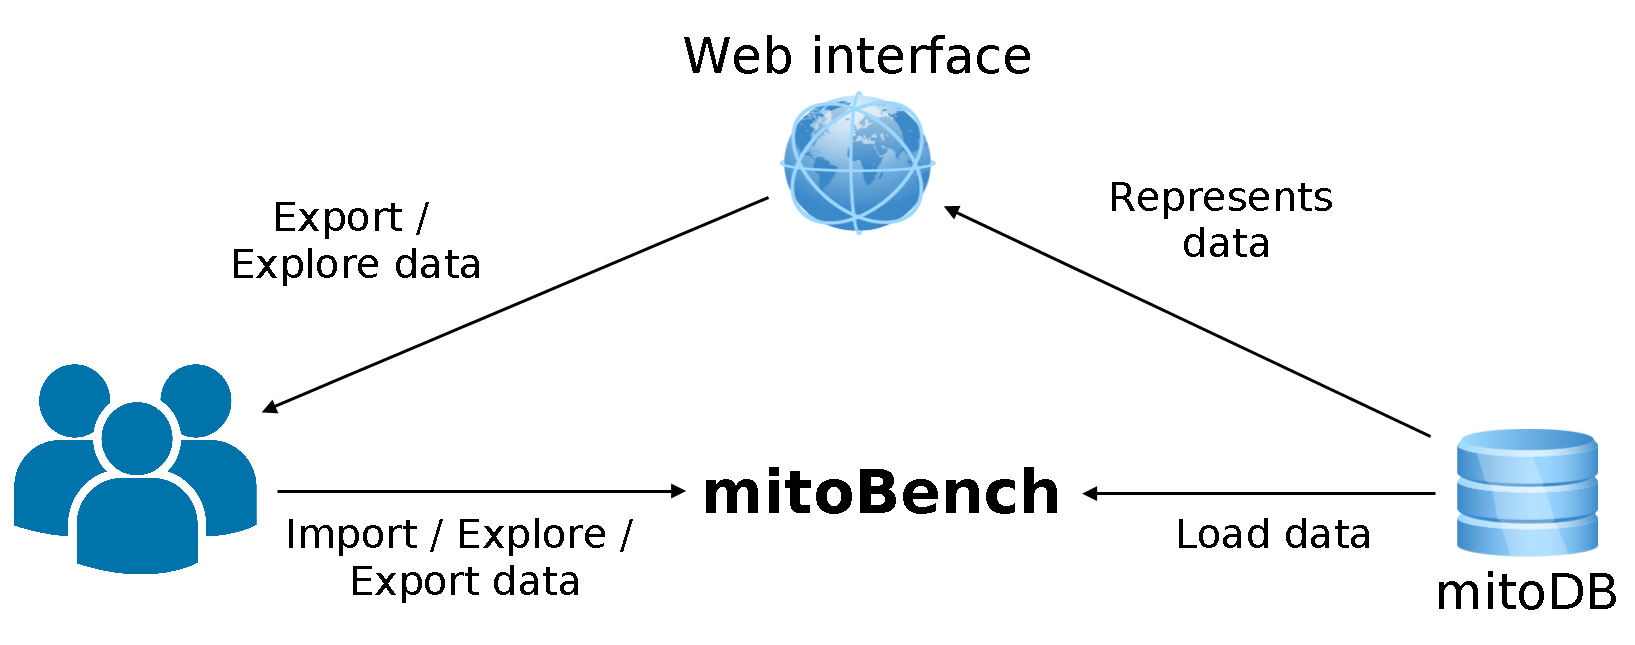
\includegraphics[width=\textwidth]{figures/workflow.png}

}

%----------------------------------------------------------------------------------------
%	MitoDB
%----------------------------------------------------------------------------------------


\headerbox{mitoDB}{name=mitodb, row=1, column=2, span=3, below=introduction, bottomaligned=workflow}{

	\begin{minipage}{0.8\textwidth}
		\begin{itemize}
			\item Database: Providing meta-information (Location, language, Sequence data, ...)
			\item Web-Frontend: Browsing data, searching for locations, quick look at database contents
			\item Data Curation: Users can rate samples in the web based on their experiences with data
			\item Access: Web-Frontend (exporting) and mitoBench (analysis)
		\end{itemize}
	\end{minipage}
	\begin{minipage}{0.15\textwidth}
		\begin{center}
			
\includegraphics[width=2cm]{figures/postgresql.png}
			\vspace{2em}
			
\includegraphics[width=0.1\paperwidth]{figures/vaadin.png}
		\end{center}
	\end{minipage}

}



%----------------------------------------------------------------------------------------
%	Mitobench
%----------------------------------------------------------------------------------------


\headerbox{mitoBench}{name=mitobench, column=0, span=3,below=workflow}{
	\begin{minipage}[t]{0.5\textwidth}
		\textbf{File conversions}\\
		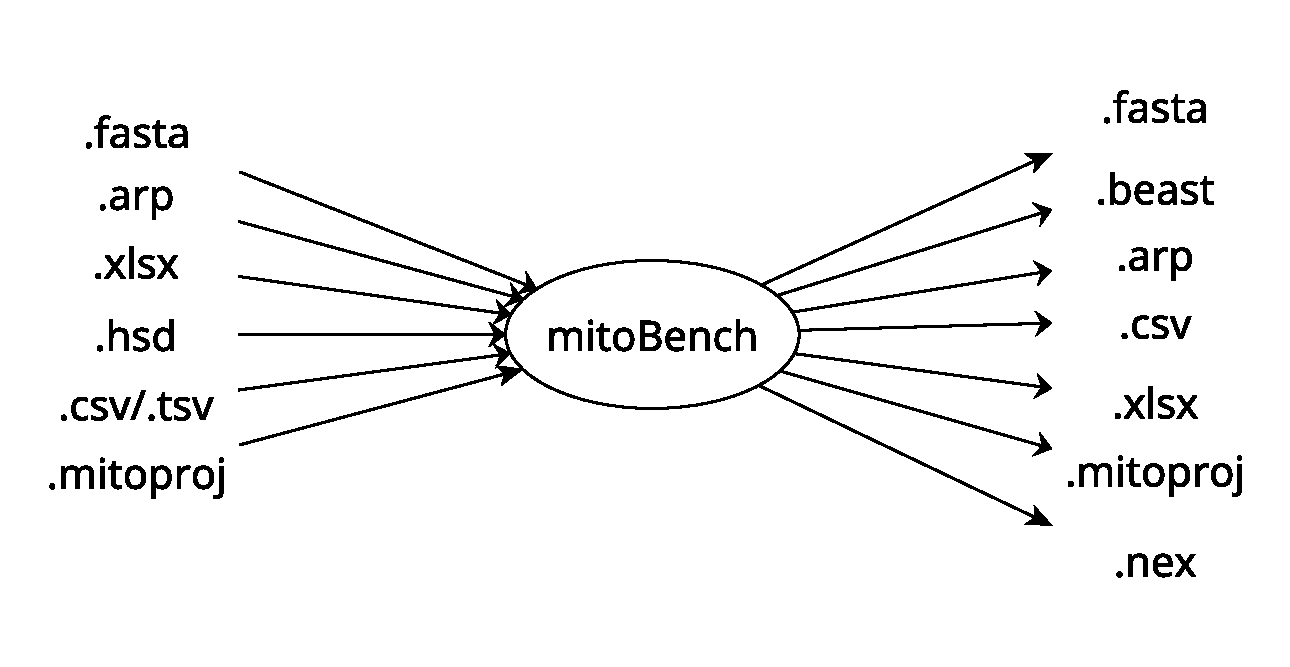
\includegraphics[width=0.9\textwidth, left]{figures/import_export.pdf}
		$\Rightarrow$ connect the workbench with existing analysis methods/resources such as BEAST$^1$, Arlequin$^2$, PhyloTree$^3$ and others
	\end{minipage}
	\hspace{0.5em}
	\begin{minipage}[t]{0.5\textwidth}
		\textbf{Data representation as Table}\\
		\\
		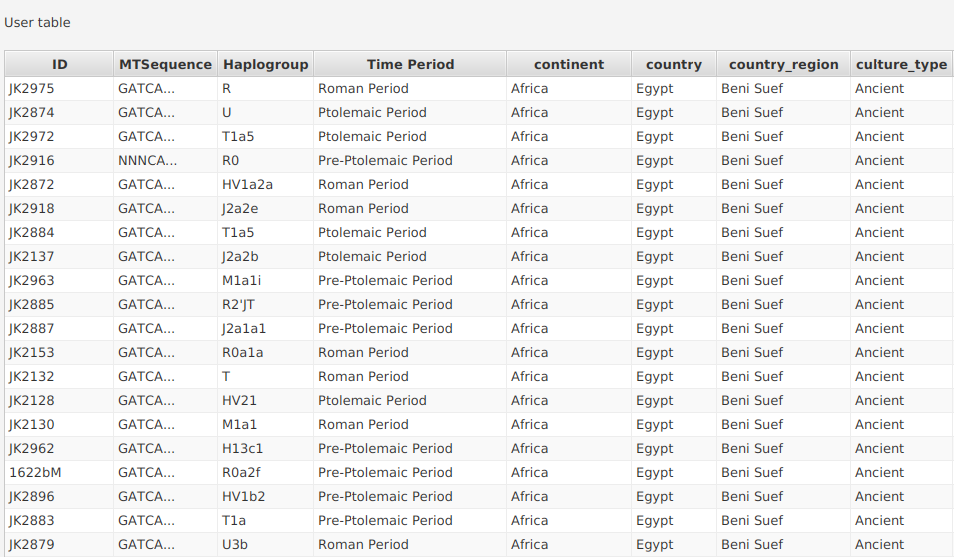
\includegraphics[width=0.85\textwidth, left]{figures/table3.png}
	\end{minipage}

	\vspace{1em}

	\begin{minipage}[t]{0.5\textwidth}
		\textbf{Data grouping}
		\begin{itemize}[leftmargin=*]
			\item group data based on shared features \\
			(e.g. time period, location)
			\item user defined grouping
		\end{itemize}
		
	\end{minipage}
	\hspace{0.5em}
	\begin{minipage}[t]{0.5\textwidth}
		\textbf{Data filtering / Statistics}
		\begin{itemize}[leftmargin=*]
			\item Haplogroup filtering / frequencies
			\item Haplotype filtering / frequencies
		\end{itemize}
		%Haplogroups based on PhyloTree.org$^3$
	\end{minipage}
\begin{center}$\Rightarrow$ allows analysis of Haplogroup distribution between different groups\end{center}
	\vspace{1em}

\textbf{Exemplary study: Analysis of 90 ancient Egyptian mummy mtDNA genomes$^4$}\\\vspace{4mm}
$\rightarrow$ Did Haplogroup frequencies change over time? If so, how?\\
\\
	\begin{minipage}{0.5\textwidth}
		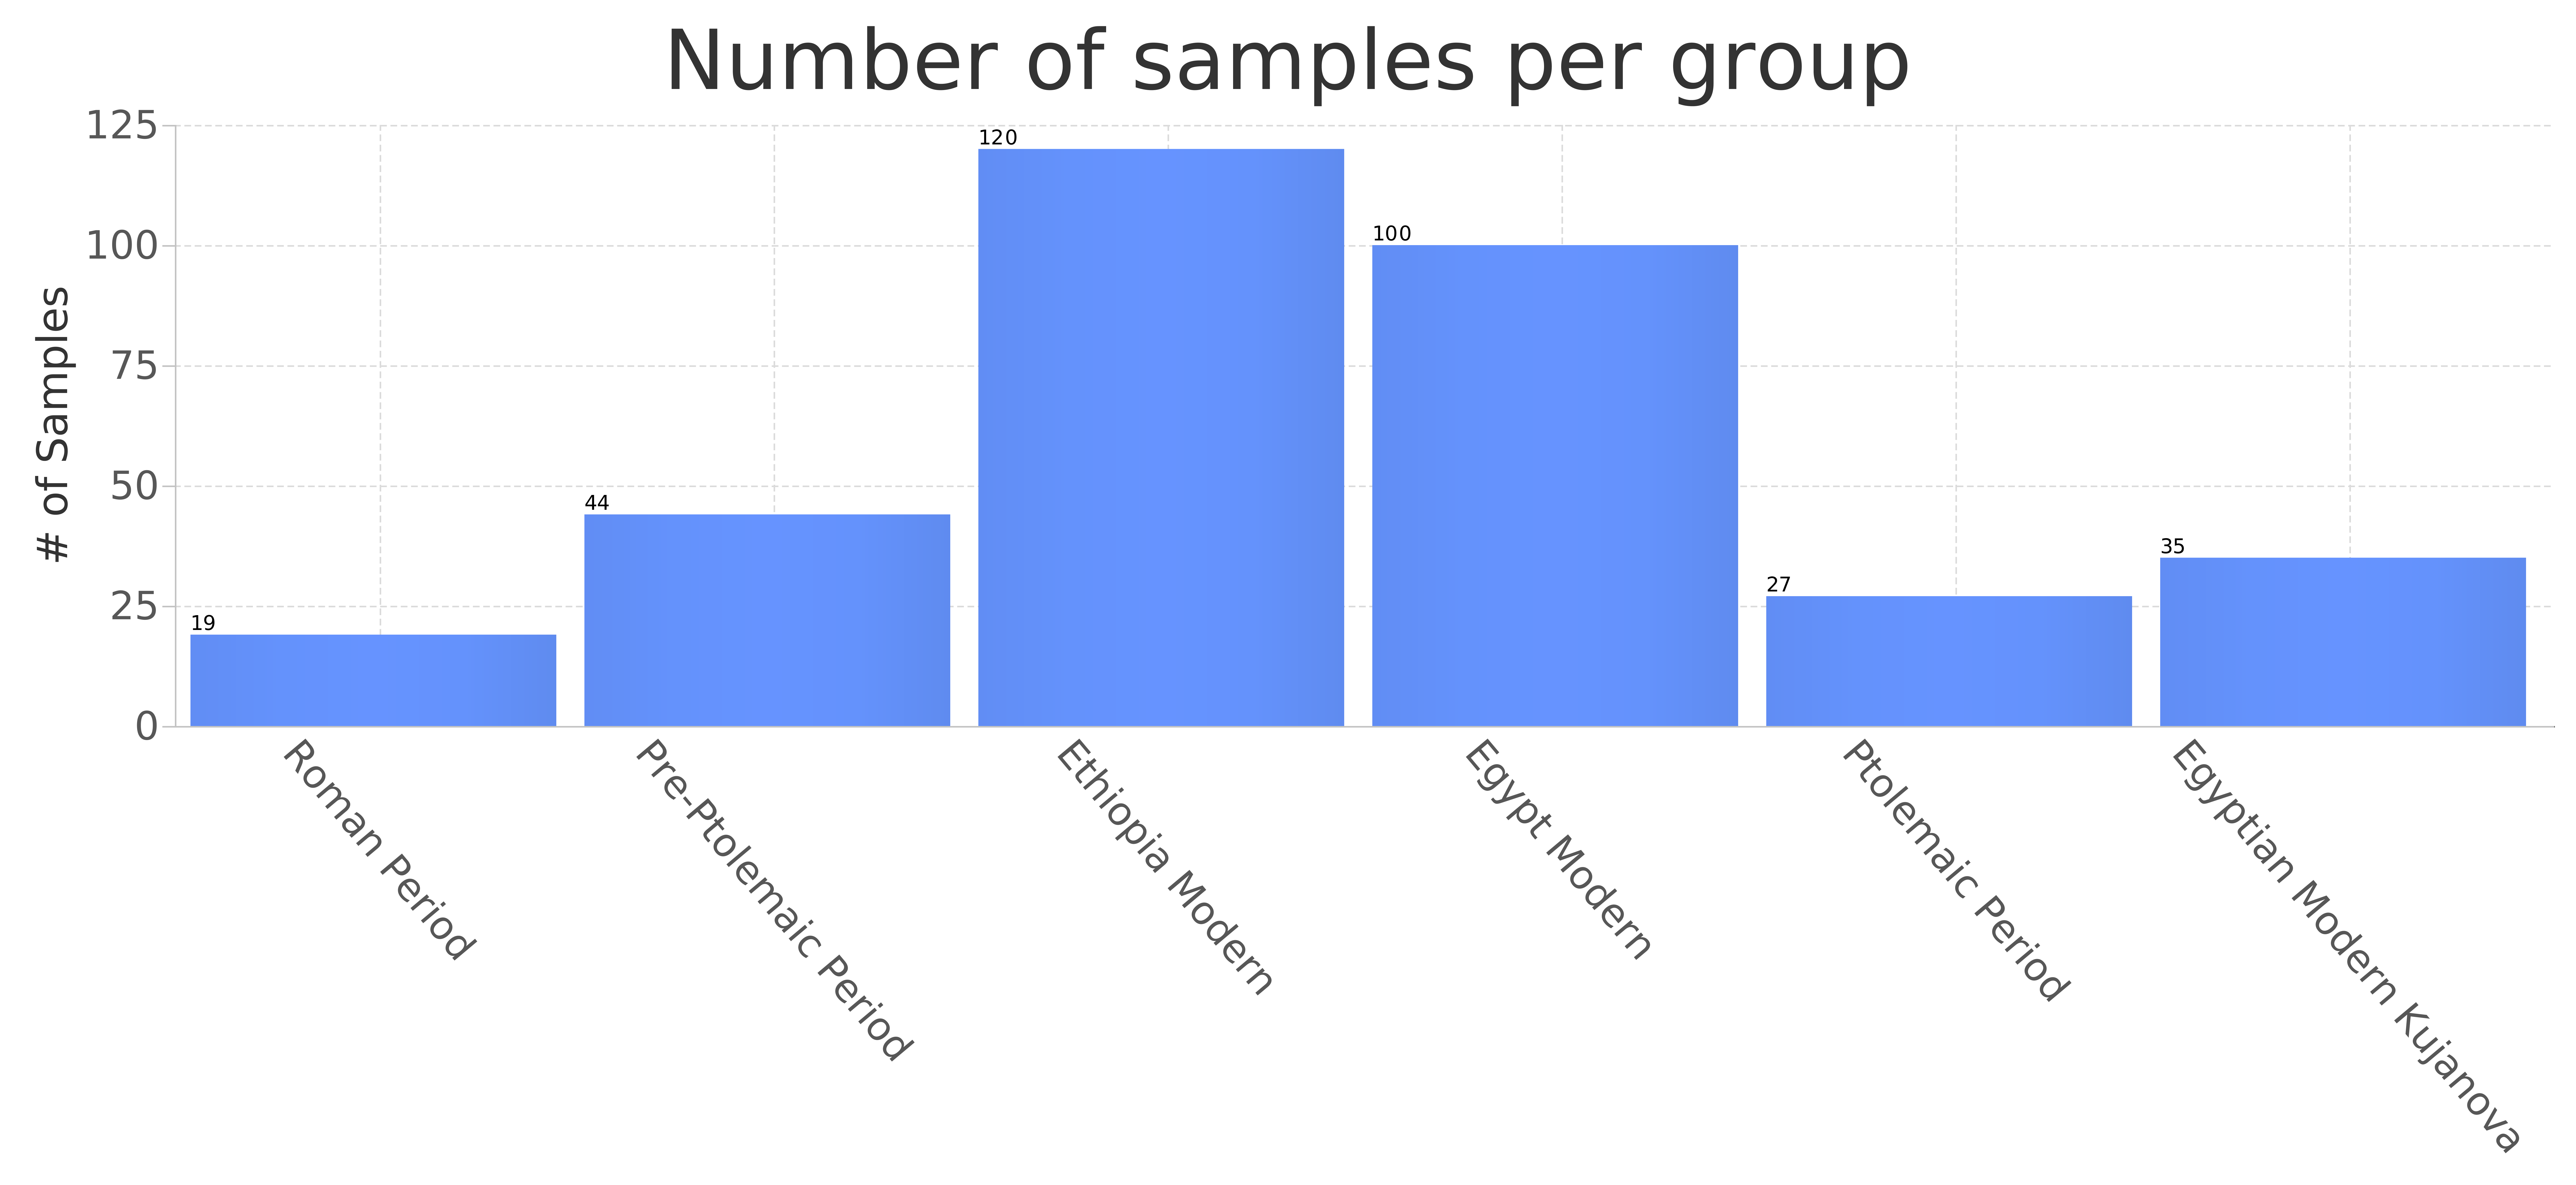
\includegraphics[width=\textwidth]{figures/group_sizes2.png}
	\end{minipage}
	\begin{minipage}{0.5\textwidth}
			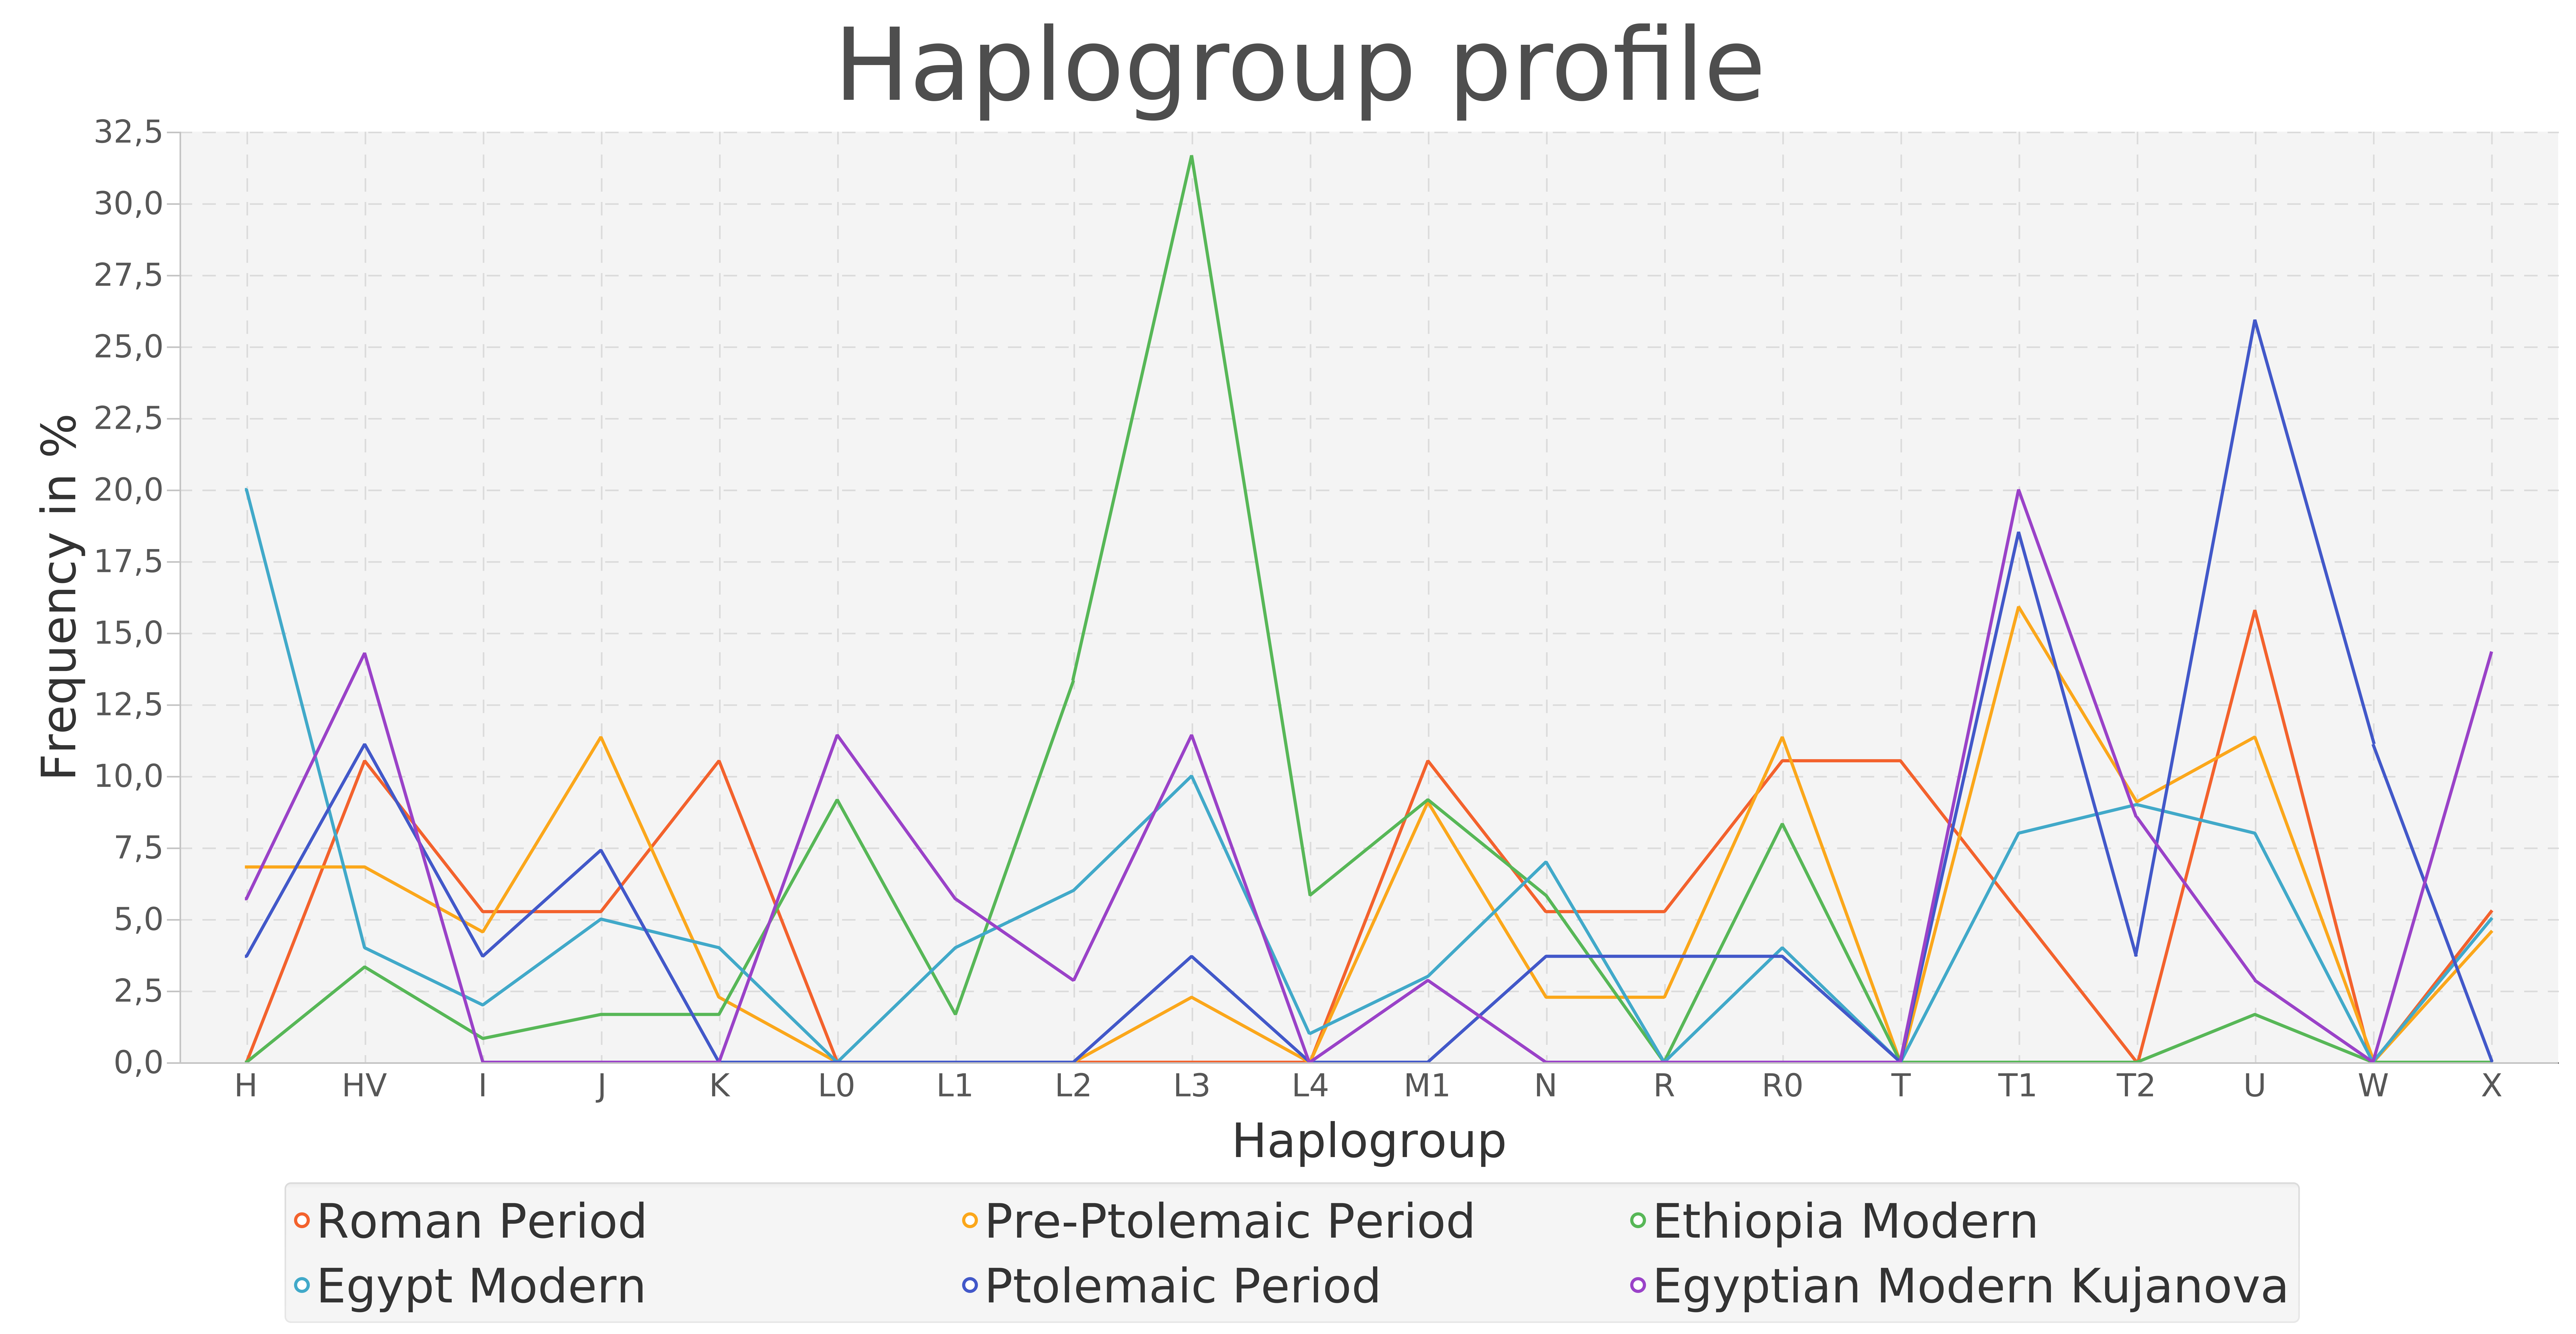
\includegraphics[width=\textwidth]{figures/profile.png}
	\end{minipage}

	\begin{minipage}{0.9\textwidth}
		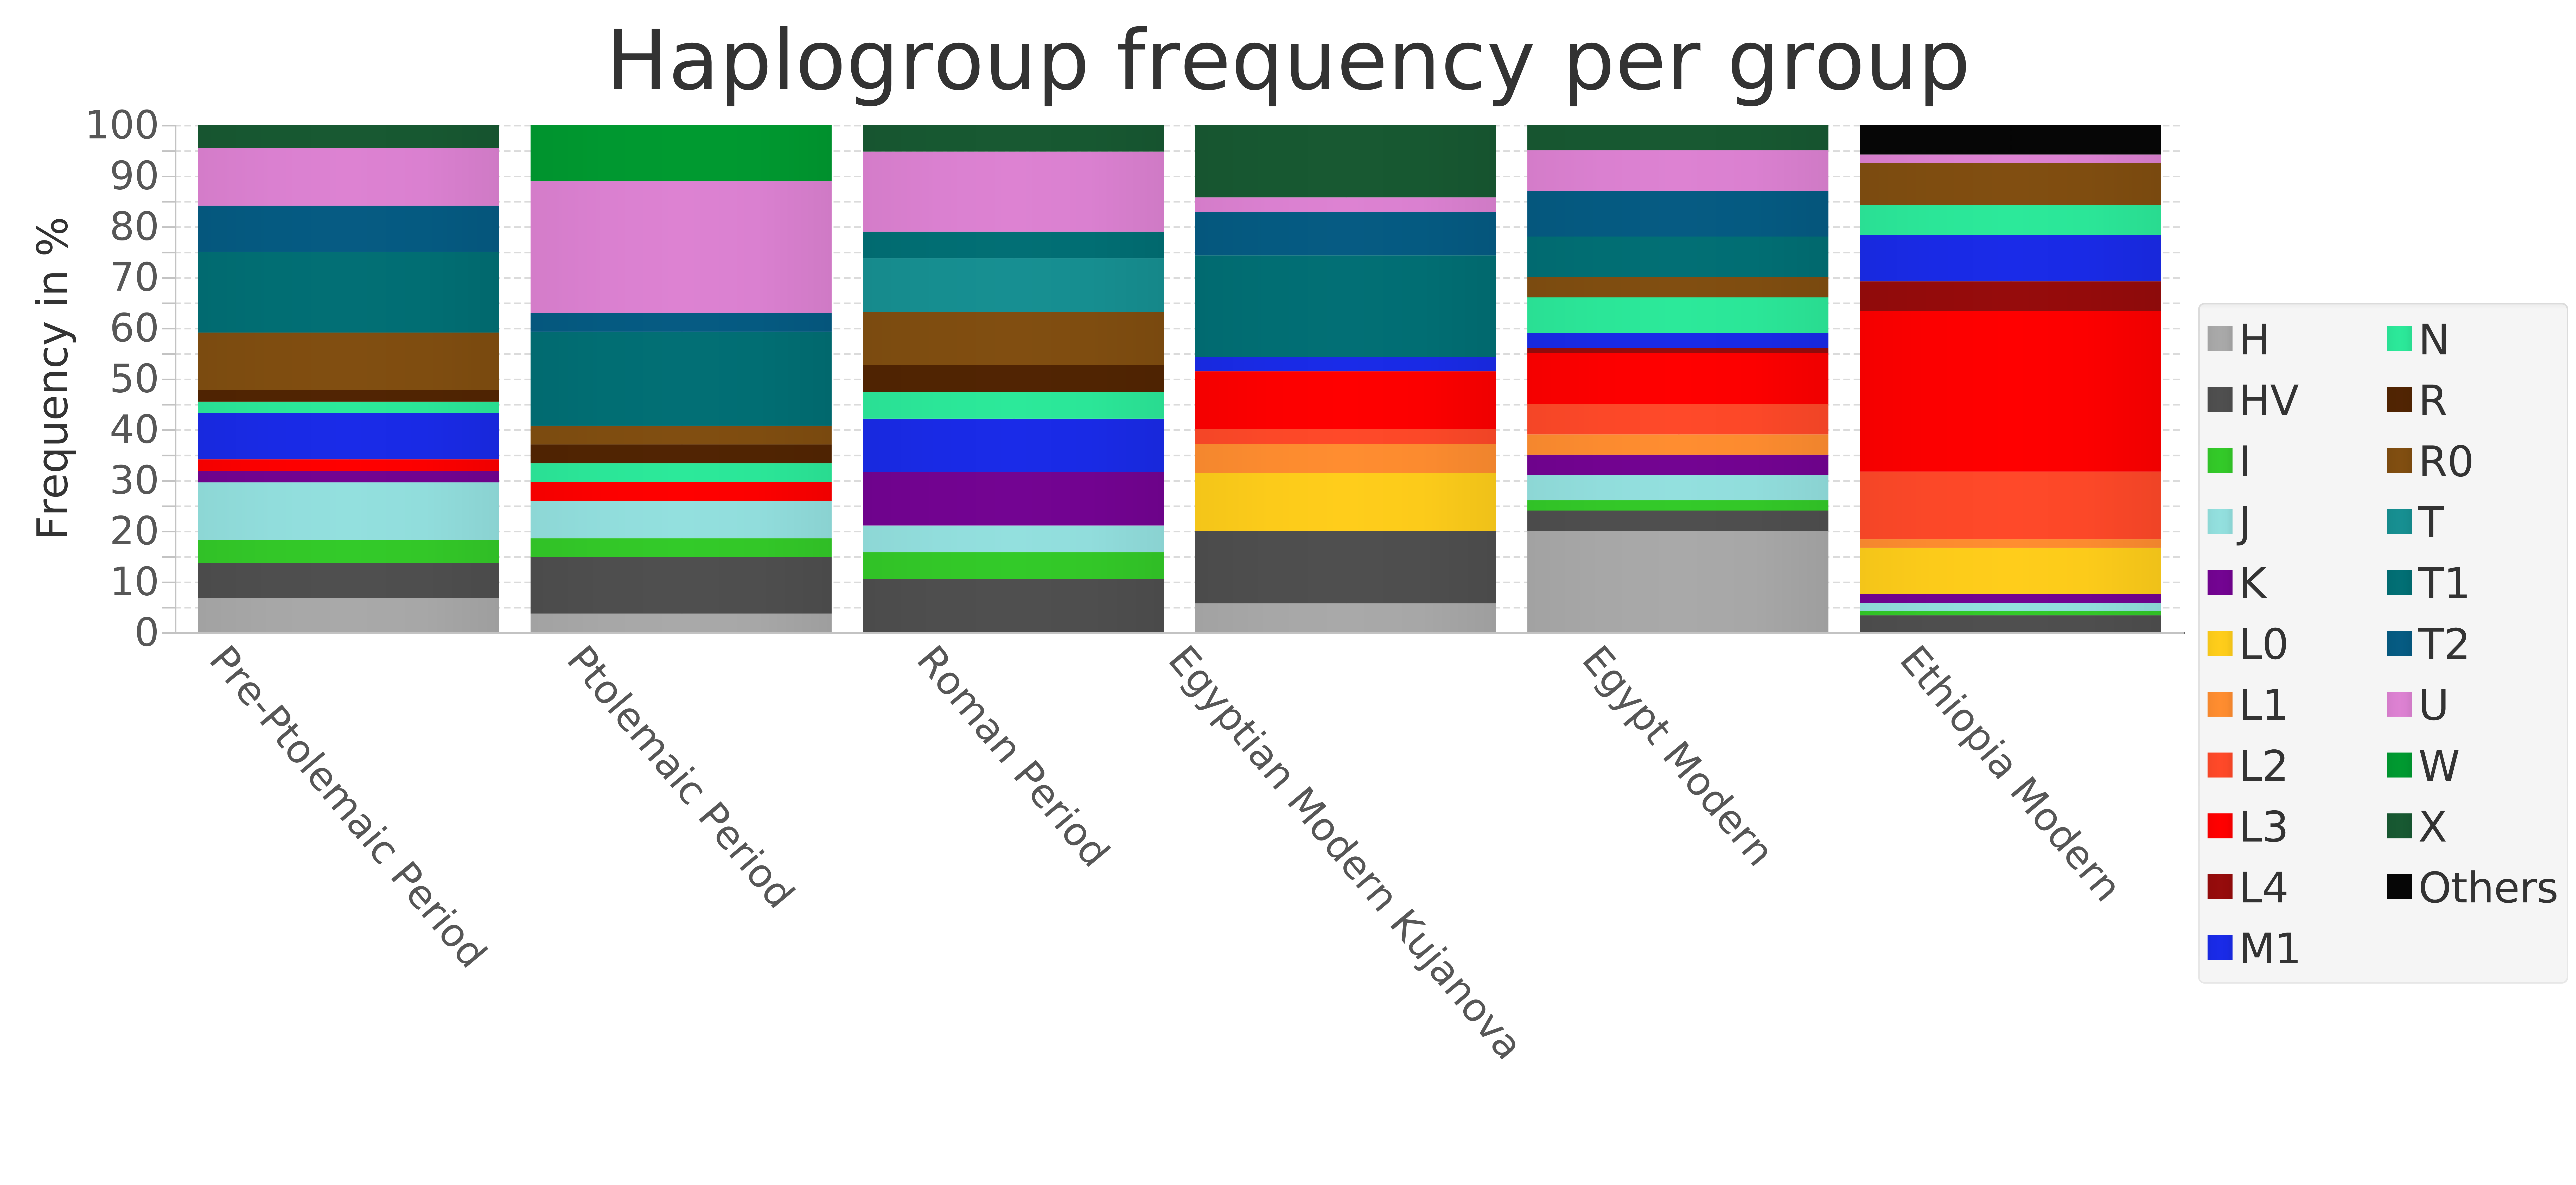
\includegraphics[width=\textwidth]{figures/stackedBarchart2.png}
	\end{minipage}
	%\begin{minipage}{0.5\textwidth}
	%	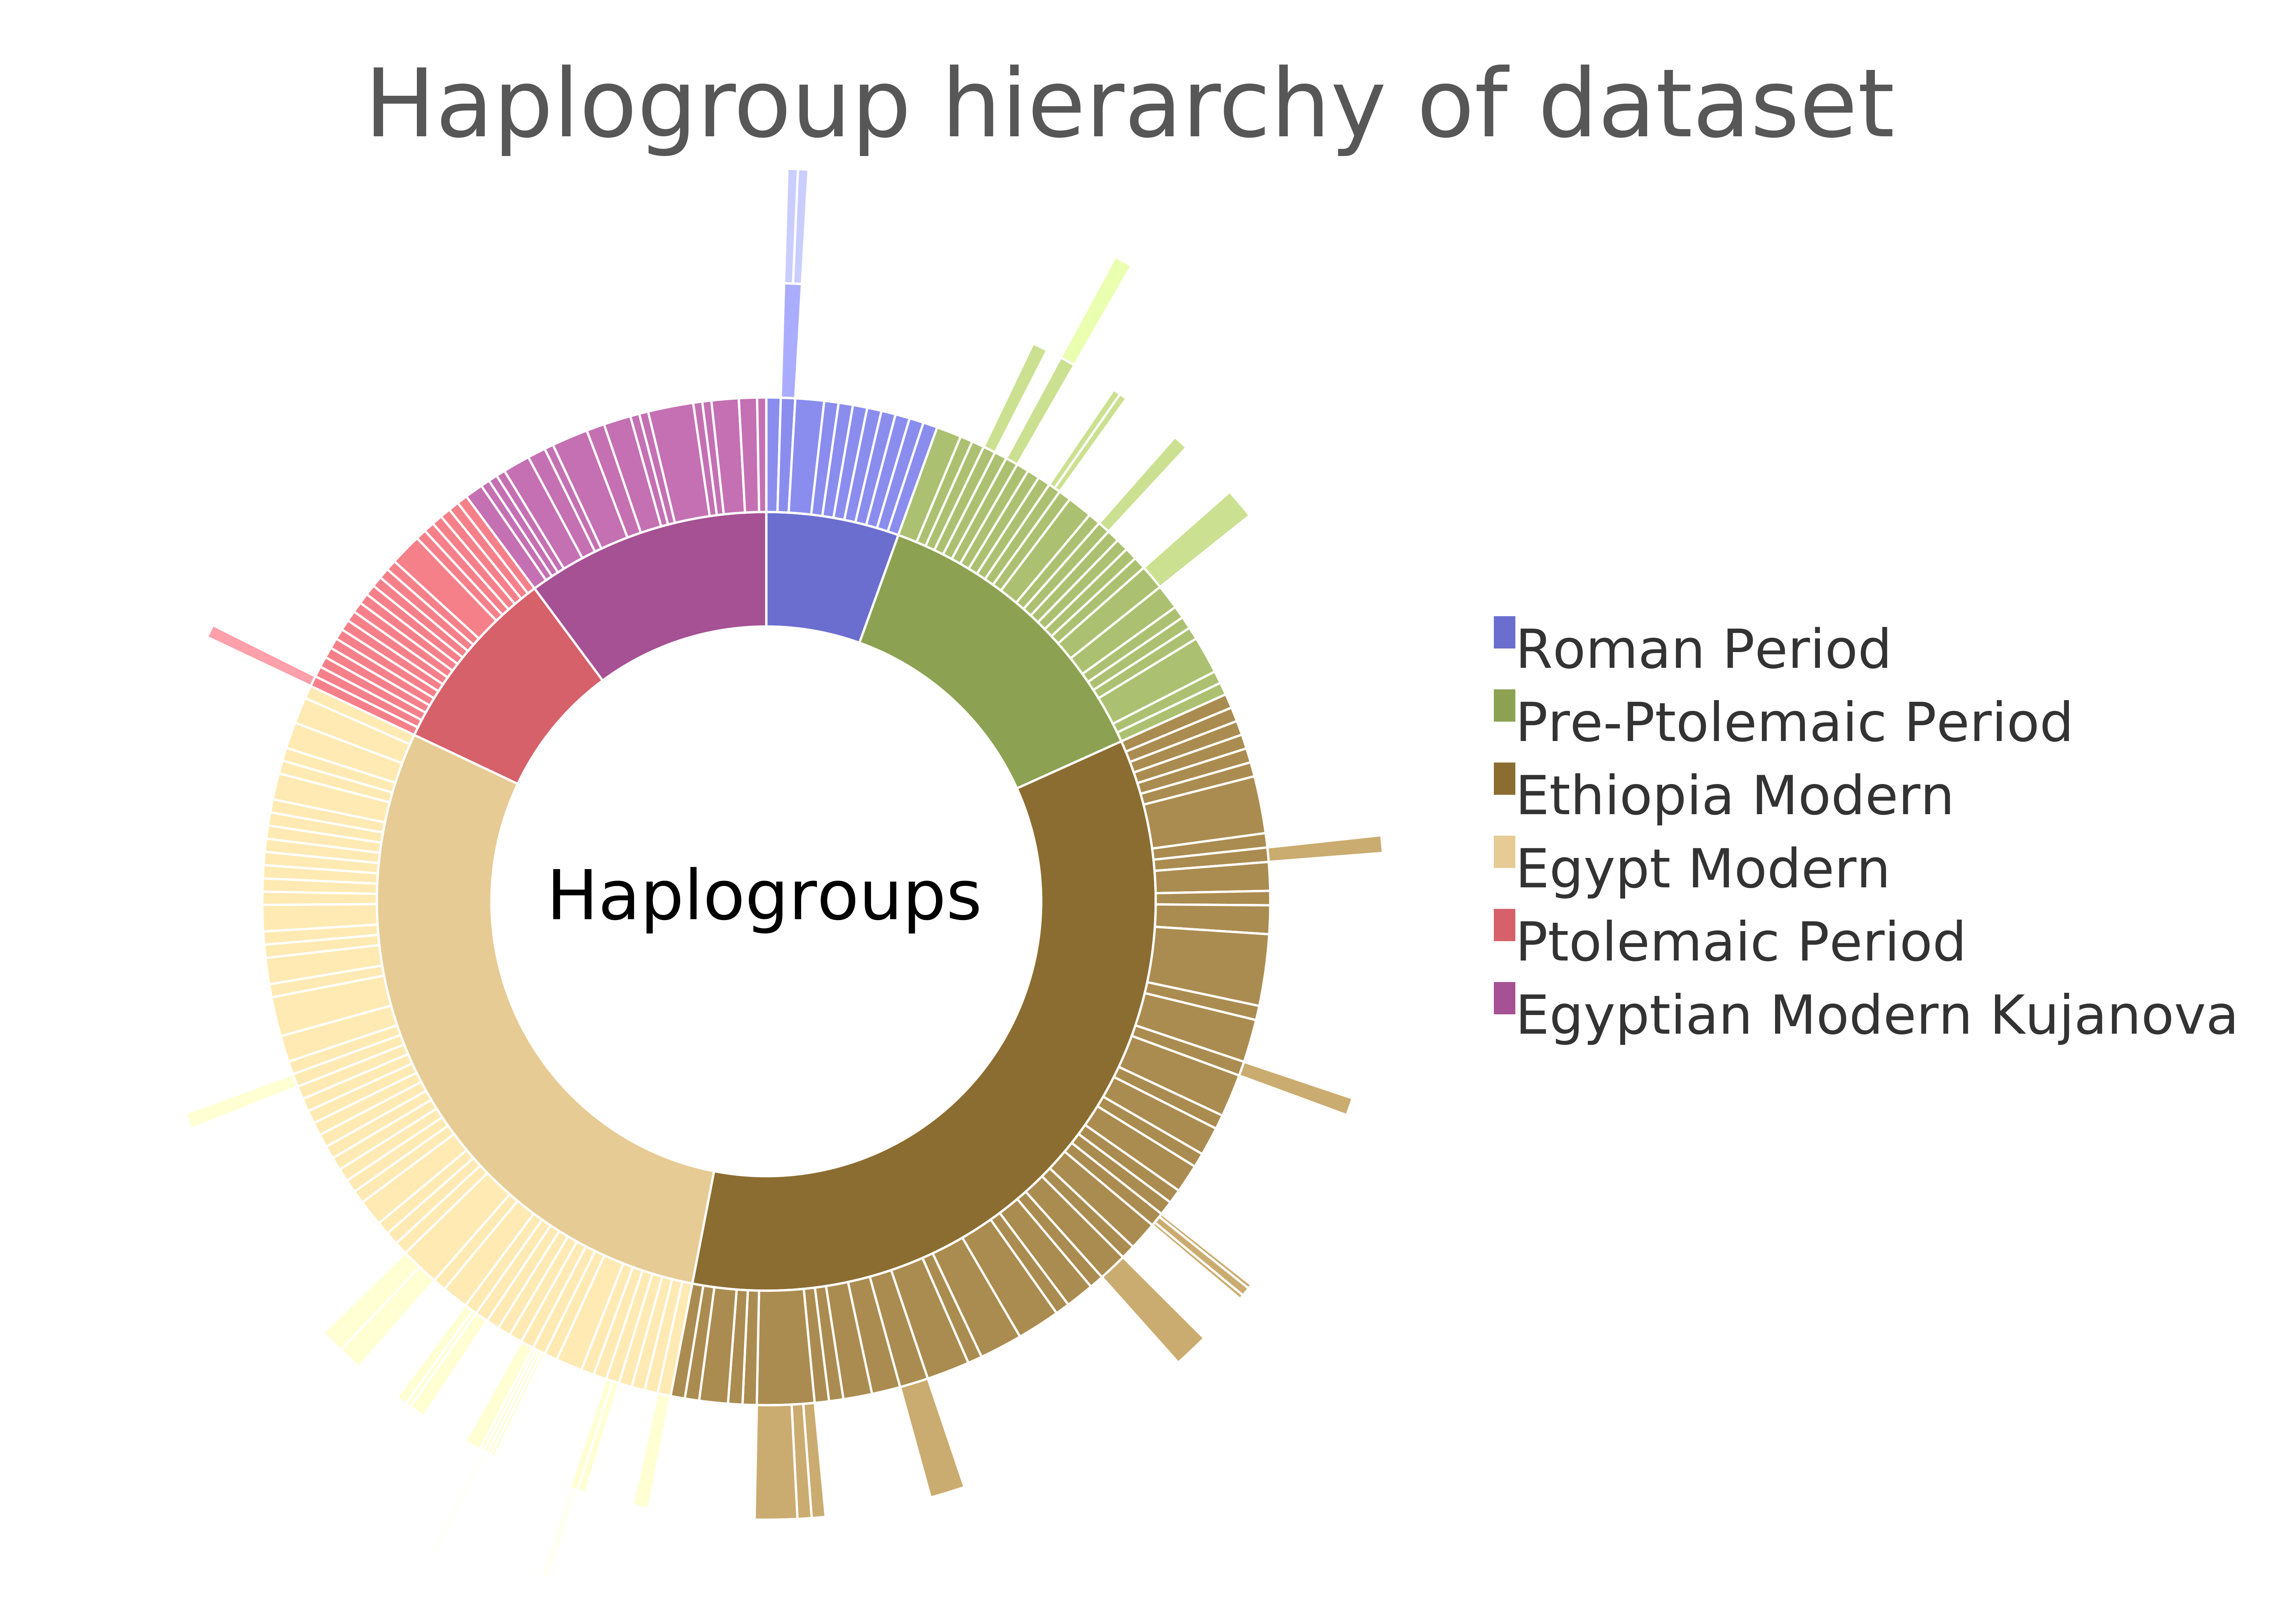
\includegraphics[width=0.8\textwidth]{figures/sunburst3.png}
	%\end{minipage}


}


%----------------------------------------------------------------------------------------
%	Outlook
%----------------------------------------------------------------------------------------

\headerbox{Outlook}{name=outlook,row=0, column=3, span=2,  below=mitodb}{
	\textbf{mitoBench}
	\begin{itemize}
		\item Provide methods for downstream analysis \\
		(e.g. F$_{ST}$ calculations, Founder Analysis)
		\item Offer more visualizations (e.g. geographical maps for origin of samples)\\
		\end{itemize}
	\begin{center}
		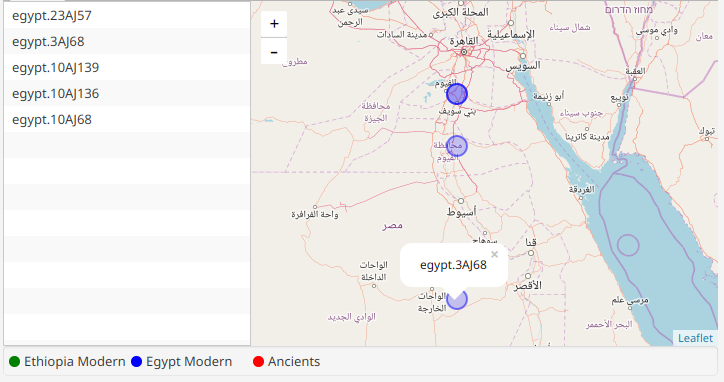
\includegraphics[width=0.7\textwidth]{figures/map2.png}
	\end{center}

	\textbf{mitoDB \& web interface}
	\begin{itemize}
		\item Export/import functionality
		\item Web-based dashboard to explore database
		\item More public datasets: 1000G, GenBank, ... 
	\end{itemize}
	\begin{center}
		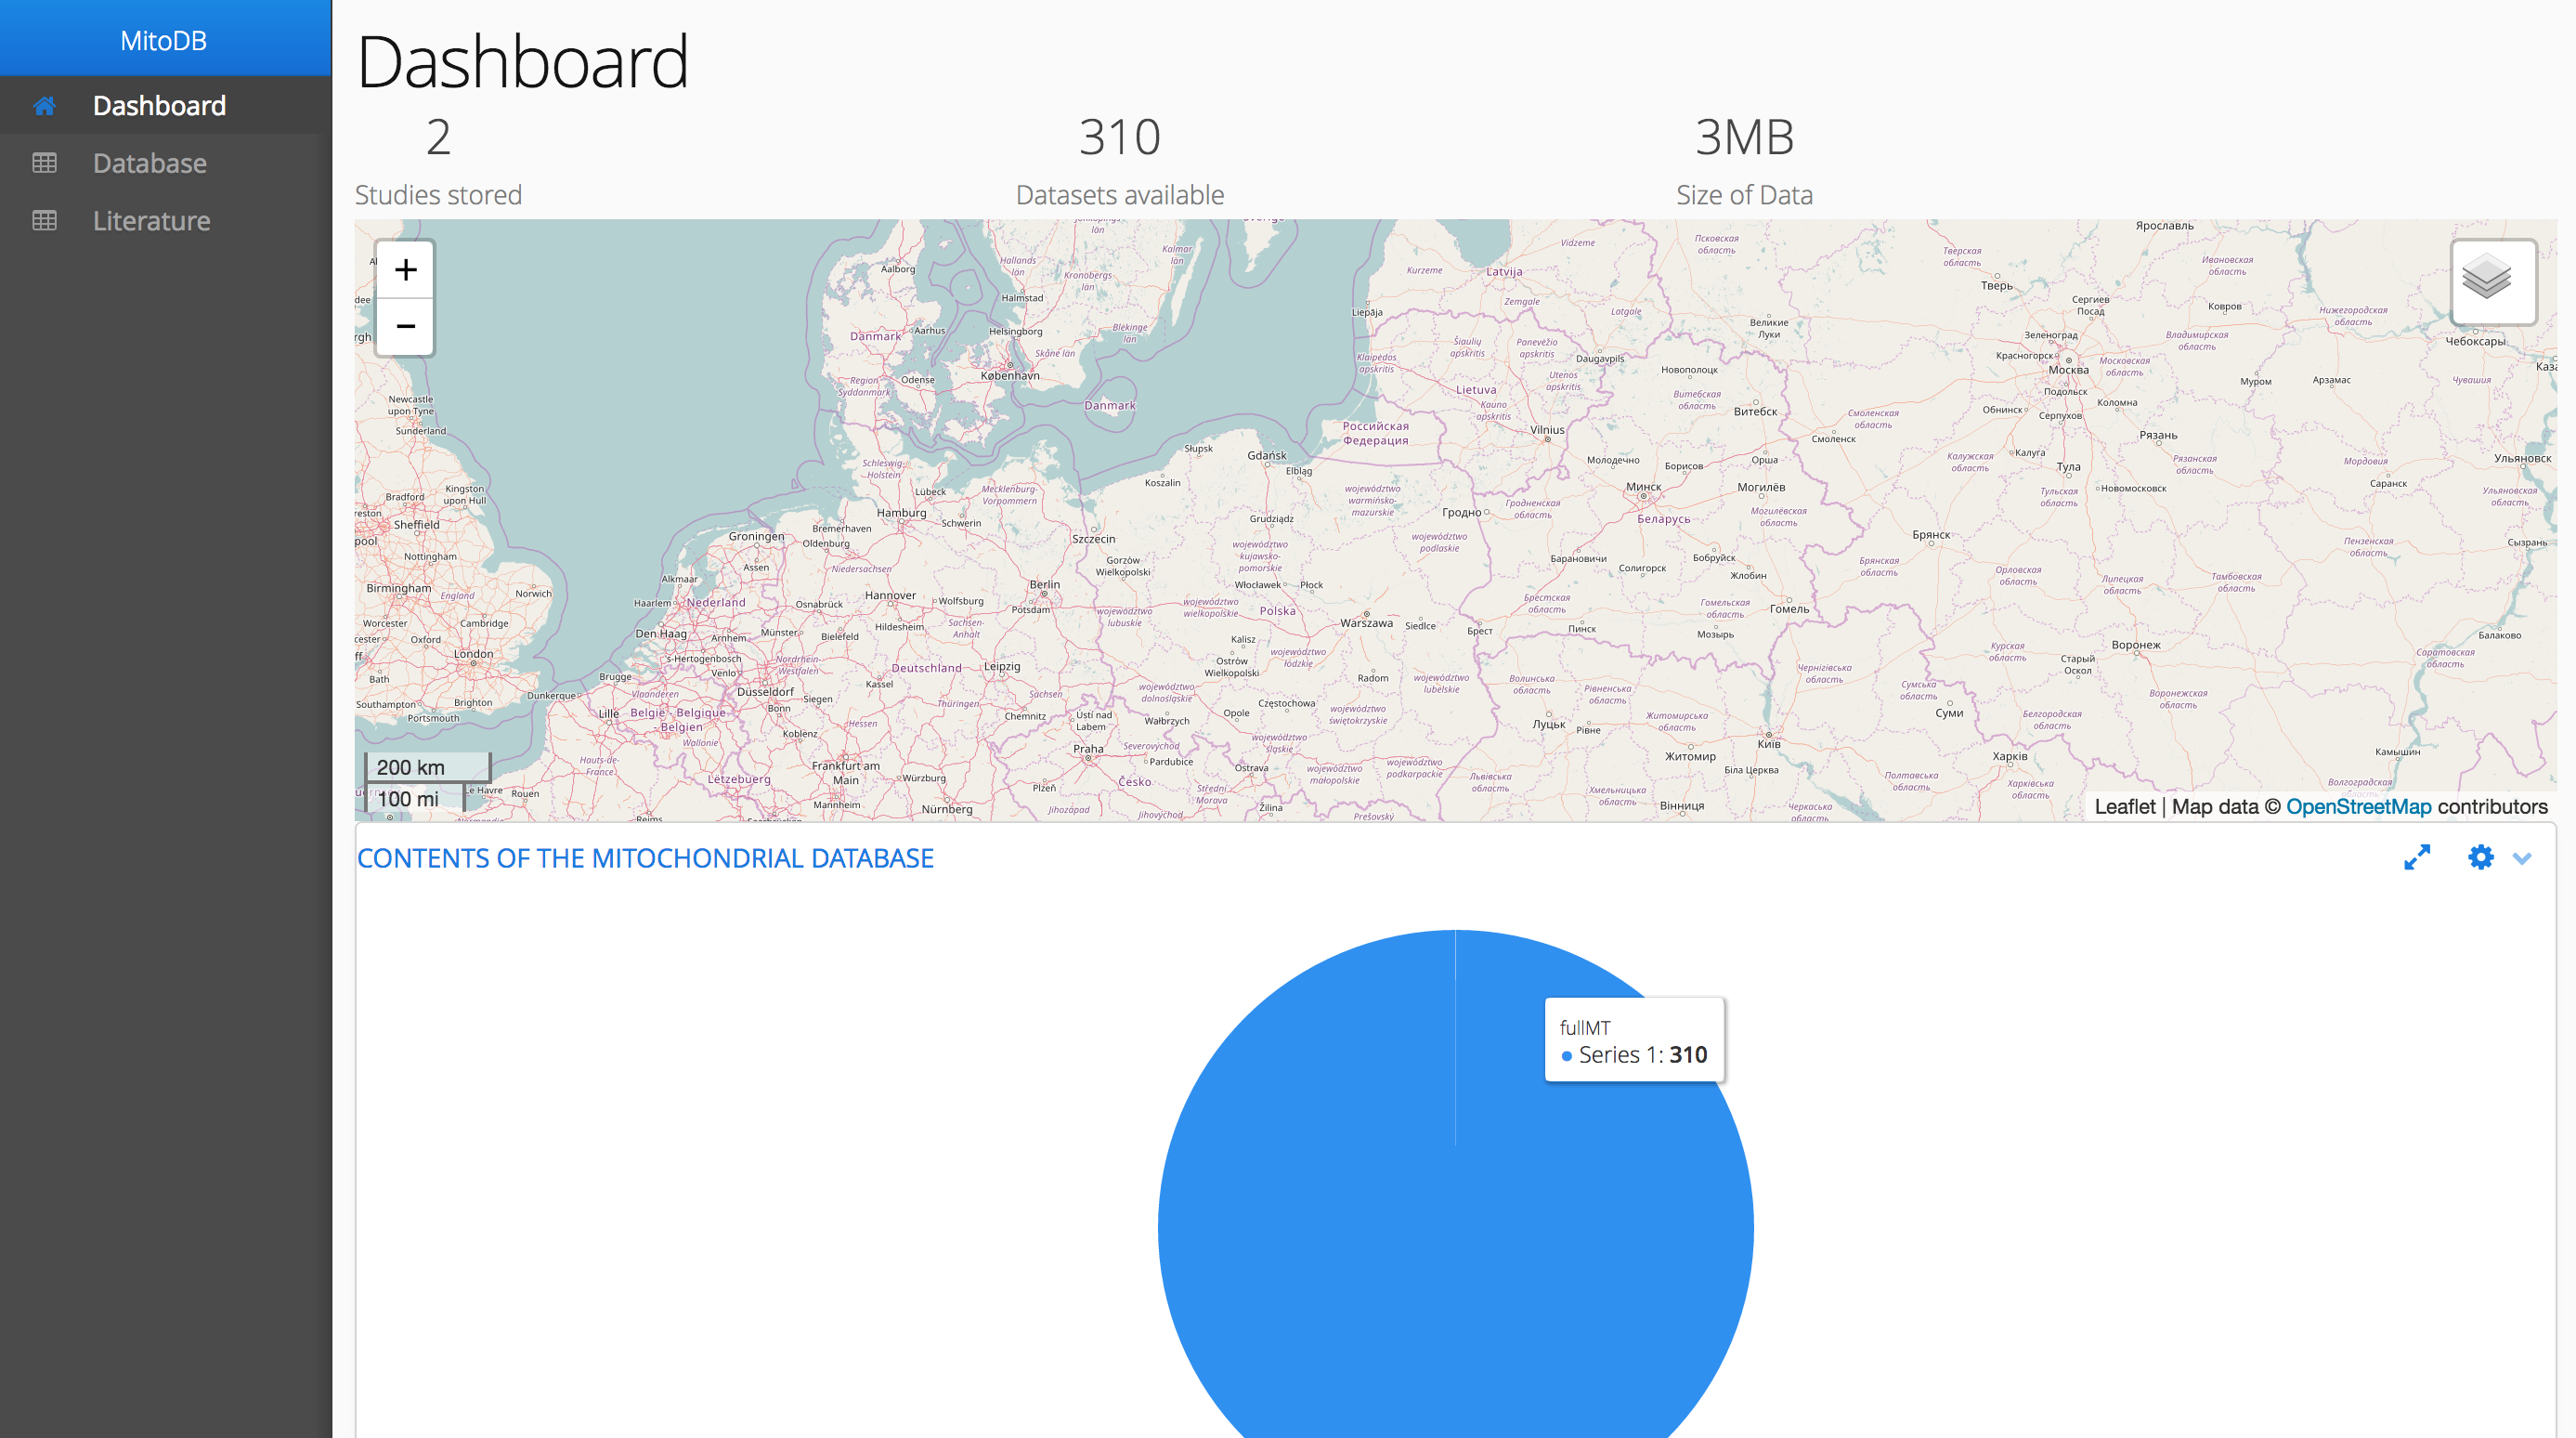
\includegraphics[width=0.7\textwidth]{figures/mitodb_dashboard.png}
	\end{center}


}


%----------------------------------------------------------------------------------------
%	References
%----------------------------------------------------------------------------------------

\headerbox{References}{name=references, column=3, span=2, above=bottom, below=outlook}{
	\scriptsize
	\begin{enumerate}[topsep=0pt,itemsep=-1ex,partopsep=1ex,parsep=1ex]
			\item Drummond, A. J.; Suchard, M. A.; Xie, D.; \& Rambaut, A. (2012). Bayesian phylogenetics with BEAUti and the BEAST. \textit{Molecular biology and evolution}, 29(8), 1969-1973.
			\item Excoffier, L. \& Lischer, H. E. (2010). Arlequin suite ver 3.5: a new series of programs to perform population genetics analyses. \textit{Molecular ecology resources}, 10(3), 564-567.
			\item Van Oven, M. \& Kayser, M. (2009). Updated comprehensive phylogenetic tree of global human mitochondrial DNA variation. \textit{Human mutation}, 30(2), E386-E394.
			\item Schuenemann, V.J. \& Peltzer, A. \textit{et. al.}. (2017). Ancient Egyptian mummy genomes suggest an increase of Sub-Saharan African ancestry in post-Roman periods. \textit{Nature Communications}, 15694. 
	\end{enumerate}
}


\end{poster}
\end{document}
